\subsection{Bounded Unfairness from Directed Bandwidth}
\label{subsec:order-fairness-from-directed-bandwidth}

Given honest transaction profiles \profileSet (with Condorcet cycles), our goal is to find an ordering that does not put $\tx'$ too early before $\tx$ when $\tx \before^\varphi \tx'$.
%
Consider a dependency graph $G \in \mathbb{G}_{\profileSet, \varphi}$ and a vertex ordering \orderOutput on $G$.
%
\cref{thm:profile-supergraph} implies that $G$ contains cycles (as all edges forming the cycles in $G_{\profileSet, \varphi}$ preserve in $G$), i.e., there will be back edges $(\tx, \tx')$ such that $\tx \before^\varphi \tx'$ and $\orderOutput(\tx) > \orderOutput(\tx')$.
%
The length of a back edge $(\tx, \tx')$ is the distance of its source and target in the ordering $\orderOutput(\tx) - \orderOutput(\tx')$.
%
Ideally, a fair order comes with back edges of small lengths.
%
In order to quantify how small the length of a back edge can be, we are interested in finding a vertex ordering on the dependency graph $G$ that minimizes the maximum length of back edges.
%
Following the similar treatment in \cite{FSTTCS:JKLSS19} (where they consider the forward edges), we state this problem as \textsc{DirectedBandwidth} in \cref{def:directed-bandwidth}.

\begin{definition}[Directed Bandwidth]
    \label{def:directed-bandwidth}

    Given a directed graph $G = (V, E)$, \textsc{DirectedBandwidth} asks to find a vertex ordering $\orderOutput^*$ such that $\DBW(\orderOutput^*, G) = \min_{\orderOutput} \DBW(\orderOutput, G)$ where
    %
    \[ \DBW(\orderOutput, G) = \max_{\substack{(u, v) \in E,\\\orderOutput(u) > \orderOutput(v)}} \orderOutput(u) - \orderOutput(v). \]
    %
    The directed bandwidth of a graph $G$ is $\DBW(G) = \DBW(\orderOutput^*, G)$.
\end{definition}

Note that when $G$ is acyclic, there exist \orderOutput which is a topological ordering on $G$ such that no back edge exists; this has little to do with the fair-order serialization problem and $\DBW(G) = 0$ for an acyclic graph.
%
We also note that $\DBW(G) = 0$ if $G$ is the null graph.

Analogous to \cref{def:directed-bandwidth}, \textsc{Bandwidth} \cite{JGT:CCDG82,SWAT:Feige00,CygPil08} is a well-known and extensively studied graph problem aiming at minimizing the quantity $\mathtt{BW}(G, \orderOutput) = \max_{(u, v)\in E} |\orderOutput(u) - \orderOutput(v)|$ among all vertex orderings on an undirected graph.
%
\textsc{Bandwidth} has been proved to be both \NP-hard \cite{Papadimitriou76} and \NP-hard to approximate within any constant ratio \cite{JCSS:DFU11} over general graphs.
%
Further, \textsc{Bandwidth} remains \NP-hard and \NP-hard to approximate even on very restricted graphs like caterpillars of hair length at most 3 (a restricted tree).

Since an undirected graph can be converted to a digraph by replacing each edge with two symmetric directed edges, there is a simple reduction from \textsc{Bandwidth} to \textsc{DirectedBandwidth} and thus \textsc{DirectedBandwidth} is also \NP-hard and \NP-hard to approximate over general graphs.
%
Notice that, in our context, dependency graphs are all oriented graphs.
%
We prove that \textsc{DirectedBandwidth} remains \NP-hard and \NP-hard to approximate within any constant ratio over oriented graphs.
%
Refer to \cref{subsec:hardness-of-directedbandwidth} for a detailed proof.

\begin{theorem}
    \textsc{DirectedBandwidth} is \NP-hard and \NP-hard to approximate within any constant ratio over oriented graphs.
\end{theorem}

\textsc{DirectedBandwidth} can be solved trivially in factorial time ($\bigO^\ast(n!)$) by an exhaustive search on all possible orderings; and, unlike some vertex ordering problems that can be solved by dynamic programming or divide-and-conquer, so far there is no evidence that these techniques also applies on \textsc{DirectedBandwidth}.
%
A recent work by Jain \textit{et al.} \cite{FSTTCS:JKLSS19} provides exponential algorithms to find the exact and approximate solutions to \textsc{DirectedBandwidth}.
%
Specifically, the exact algorithm runs in $\bigO^\ast(3^{|V|} \cdot 2^{|E|})$ time; and in order to get an ordering with bandwidth at most $(1 + \epsilon)$ times the optimal one, an approximation algorithm runs in $\bigO^\ast(4^{|V|} \cdot (4 / \epsilon)^{|V|})$ time.
%
We briefly describe the exact algorithm for \textsc{DirectedBandwidth} in \cref{subsec:exact-algorithm-directed-bandwidth}.

\paragraph{Largest possible directed bandwidth.}
%
Since all oriented graphs can be generated by profiles, we are interested in the largest possible bandwidth on graphs with a fixed number of vertices.

Note that, given $n$ vertices, the worst bandwidth $n - 1$ can always be avoided by finding an edge $(i, j)$ and outputting \orderOutput such that $\orderOutput(i) = 1$ and $\orderOutput(j) = n$.
%
And, for a small constant $k$, we can check if a graph has bandwidth $n - k$ by checking $\bigO(n^{2k})$ vertex orderings --- i.e., we select $k$ vertices each at the head and rear of orderings and see if a back edge exists between the two sets.
%
Unfortunately, the time complexity of this simple approach grows to factorial when $k = \Theta(n)$ hence it becomes impractical for large graphs.
%
This raises the question whether it is possible to find a vertex ordering with directed bandwidth, e.g., $0.99 n$, for any oriented graph with $n$ vertices.

Here we give a negative answer to this question.
%
We prove that, among all oriented graphs with $n$ vertices there exist some tournaments with large directed bandwidth compared with $n$\footnote{This result implies that no algorithm can guarantee finding a vertex ordering of directed bandwidth $0.99n$.}.
%
In \cref{thm:largest-possible-dbw} we show that the above simple approach to check bandwidth will soon terminate on some graphs by considering Zarankiewicz's problem.
%
See \cref{subsec:upper-bound-on-worst-case-directed-bandwidth} for a detailed proof.

\begin{theorem} \label{thm:largest-possible-dbw}
    Let $\mathbb{G}_n$ denote the set of all oriented graphs with $n$ vertices.
    %
    It holds that
    %
    \[ n - 4\log n < \max_{G \in \mathbb{G}_n} \DBW(G) < n - \log n / 2.\]
\end{theorem}

\paragraph{$(\varphi, \DBW)$-fair-order.}
%
After extracting the directed bandwidth of a graph in \cref{def:directed-bandwidth}, we are now ready to define fair order based on upper-bounding how much $\tx'$ can be ordered before $\tx$ when $\tx \before^\varphi \tx'$.

Note that, given a transaction profile set \profileSet and its dependency graph $G$, we cannot simply define the upper bound as $\DBW(G)$.
%
This is because $G$ might contain several strongly connected components and their sizes might differ a lot.
%
Actually, the bandwidth of a graph $G$ is the maximum bandwidth among all strongly connected components in $G$.
%
\[  \DBW(G) = \max \{ \DBW(G') : G' \text{ is a strongly connected component of } G \}. \]
%
Suppose there is a SCC that contains thousands of transactions and $\DBW(G)$ is also in the thousands.
%
Then, for other relatively small SCCs with, for instance, 10 transactions, an upper bound as $\DBW(G)$ does not set any limitation on how they should be ordered.

Additionally, note that when given $\profileSet^\honestPartySet$ and $\varphi$, a fair-order serialization should consider all possible dependency graphs $\mathbb{G}_{\profileSet^\honestPartySet, \varphi}$ with admissible $\profileSet^\adv$.
%
\cref{thm:profile-supergraph} shows that \adv may create new cycles or enlarge existing ones, but \adv cannot remove any edge that has already been there in $G_{\profileSet^\honestPartySet, \varphi}$.
%
Due to the above observations, we propose a fine-grained definition of order fairness (\cref{def:varphi-dbw-order-fairness}) on top of \cref{def:varphi-b-order-fairness} by replacing the initial function with largest \DBW on all possible SCCs.
%
Specifically, for a pair of transaction $\tx \before^\varphi \tx'$, if among all possible dependency graphs $\mathbb{G}_{\profileSet^\honestPartySet, \varphi}$ there is no graph with SCC that contains $\tx, \tx'$ simultaneously then the final output should follow $\tx \before \tx'$.
%
Otherwise, we will define the upper bound on their distance in the output by extracting all SCCs containing $\tx, \tx'$ over $\mathbb{G}_{\profileSet^\honestPartySet, \varphi}$ and find the largest possible bandwidth.

\begin{definition}[$(\varphi, \DBW)$-fair-order]
    \label{def:varphi-dbw-order-fairness}

    A profile \orderOutput is a $(\varphi, \DBW)$-fair-order on \profileSet if for all $\tx, \tx'$ such that $\tx \before^\varphi_\profileSet \tx'$, it holds that
    %
    \[ \orderOutput(\tx) - \orderOutput(\tx') \le \max_{G \in \mathbb{G}_{\profileSet, \varphi}} \DBW \big( \SCC(G, \tx, \tx') \big), \]
    %
    where $\SCC(G, \tx, \tx')$ is a function that outputs an SCC in $G$ that contains both $\tx, \tx'$ if it exists, and a null graph otherwise.
\end{definition}

Note that in an all honest setting, no $\profileSet^\adv$ exists, thus \cref{def:varphi-dbw-order-fairness} can be simplified as ``$\tx \before^\varphi \tx' \implies \orderOutput(\tx) - \orderOutput(\tx') \le \DBW (\SCC(G_{\profileSet, \varphi}, \tx, \tx'))$''.
%
See below for an example where we have 8 transactions in \profileSet and the $(\profileSet, \varphi)$-dependency-graph is illustrated in \cref{fig:optimal-bandwidth-order}(a).
%
Since $\DBW(G_{\profileSet, \varphi}) = 3$, a $(\varphi, \DBW)$-fair-order on \profileSet should satisfy $\tx \before^\varphi \tx' \implies \orderOutput(\tx) - \orderOutput(\tx') \le 3$.
%
We provide a profile $\orderOutput = \tx_2 \before \tx_3 \before \tx_1 \before \tx_5 \before \tx_6 \before \tx_8 \before \tx_4 \before \tx_7$ which is a fair order on \profileSet in Figure~\cref{fig:optimal-bandwidth-order}(b).
%
Note that only back edges are illustrated and the back edges $(5, 2)$, $(4, 5)$ and $(8, 1)$ are of maximum length $3$.
%
Also compare with the lexicographic order which has a back edge of length $7$ (\textsf{Aequitas} and \textsf{Themis} may output this order, see below for comparison with existing protocols).

\begin{figure}[ht]
    \begin{tabularx}{\linewidth}{Y Y}
        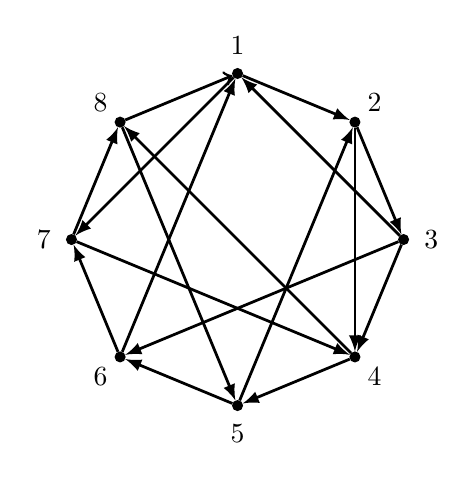
\begin{tikzpicture}
            \foreach \angle [count = \xi] in {90, 45, ..., -235}
                {
                    \node[circle, fill, minimum size=.4em, inner sep=0pt, outer sep=0pt] (node\xi) at (\angle:6em) {};
                    \node (nodetext\xi) at (\angle:7em) {\xi};
                }
            \foreach \xi in {2, 3, ..., 8}
                {
                    \pgfmathtruncatemacro\xii{\xi - 1};
                    \draw[-latex,line width = .1em] (node\xii) -- (node\xi);
                }
            \draw[->,line width = .1em] (node8) -- (node1);
            \foreach \x/\y in {3/1, 5/2, 2/4, 3/6, 8/5, 1/7, 7/4, 6/1, 4/8}
                {
                    \draw[-latex, line width = .1em] (node\x) -- (node\y);
                }
        \end{tikzpicture}
         &
        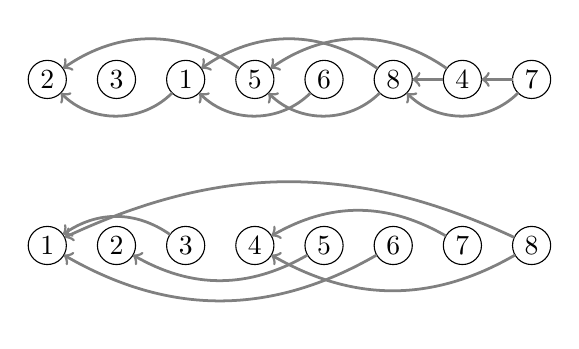
\begin{tikzpicture}
            \node[circle, fill = white, draw = black, inner sep = .2em, outer sep=0pt] (node2) {2};
            \foreach \xi [count = \xii] in {3, 1, 5, 6, 8, 4, 7}
                {
                    \pgfmathsetmacro\dist{\xii * 2.5};
                    \node[circle, fill = white, draw = black, inner sep = .2em, outer sep=0pt] at ([xshift = \dist em]node2)(node\xi) {\xi};
                }
            \draw[bend right = 35, ->, line width = .1em, gray]  (node5) to node [auto] {} (node2);
            \draw[bend left = 45, ->, line width = .1em, gray]  (node8) to node [auto] {} (node5);
            \draw[->, line width = .1em, gray] (node7) -- (node4);
            \draw[->, line width = .1em, gray] (node4) -- (node8);
            \draw[bend left = 45, ->, line width = .1em, gray]  (node6) to node [auto] {} (node1);
            \draw[bend left = 45, ->, line width = .1em, gray]  (node1) to node [auto] {} (node2);
            \draw[bend right = 35, ->, line width = .1em, gray]  (node4) to node [auto] {} (node5);
            \draw[bend left = 45, ->, line width = .1em, gray]  (node7) to node [auto] {} (node8);
            \draw[bend right = 35, ->, line width = .1em, gray]  (node8) to node [auto] {} (node1);

            \node[circle, fill = white, draw = black, inner sep = .2em, outer sep=0pt] at ([yshift = -6em]node2) (node21) {1};
            \foreach \xi [count = \xii] in {2, 3, ..., 8}
                {
                    \pgfmathsetmacro\dist{\xii * 2.5};
                    \node[circle, fill = white, draw = black, inner sep = .2em, outer sep=0pt] at ([xshift = \dist em]node21)(node2\xi) {\xi};
                }

            \draw[bend left = 30, ->, line width = .1em, gray]  (node25) to node [auto] {} (node22);
            \draw[bend right = 35, ->, line width = .1em, gray]  (node23) to node [auto] {} (node21);
            \draw[bend left = 30, ->, line width = .1em, gray]  (node26) to node [auto] {} (node21);
            \draw[bend right = 30, ->, line width = .1em, gray]  (node27) to node [auto] {} (node24);
            \draw[bend right = 25, ->, line width = .1em, gray]  (node28) to node [auto] {} (node21);
            \draw[bend left = 30, ->, line width = .1em, gray]  (node28) to node [auto] {} (node24);
        \end{tikzpicture}
        \\
        (a) dependency graph $G_{\profileSet, \varphi}$ \linebreak
         &
        (b) $(\varphi, \DBW)$-fair-order (above) and lexicographic order (below)
        \\
    \end{tabularx}
    \addtocounter{table}{-1}
    \medskip

    \caption{Illustration of a dependency graph, a $(\varphi, \DBW)$-fair-order and a lexicographic order on \profileSet. Only back edges are illustrated in (b).}
    \label{fig:optimal-bandwidth-order}
\end{figure}

We highlight that \cref{def:varphi-dbw-order-fairness} is the most precise definition that we can make on top of \cref{def:varphi-b-order-fairness,def:fair-order-serialization}.
%
For any new definition that tries to further reduce $\max_{G \in \mathbb{G}_{\profileSet, \varphi}} \DBW(\SCC(G, \tx, \tx'))$ for transactions $\tx, \tx'$, there will exist some profiles $\profileSet^\adv$ leading to SCCs with large bandwidth which can invalidate the new definition.
%
Refer to \cref{sec:discussions} for further discussions.

\begin{theorem} \label{thm:best-fairness}
    Suppose that a protocol implements $(\varphi, B)$-fairness for a function $B$.
    %
    Then for all \profileSet there are $\tx,\tx'$ with $\tx \before^\varphi \tx'$,  such that $B$ satisfies
    %
    \( B(\profileSet, \varphi, \tx, \tx') \allowbreak \geq \max_{G \in \mathbb{G}_{\profileSet, \varphi}} \DBW (\SCC(G, \tx, \tx')) \).
\end{theorem}

\begin{proof}
    Fix an order fairness parameter $\varphi$.
    %
    Towards a contradiction, suppose there exist a function $B$ such that $\exists \profileSet, \forall(\tx, \tx'), B(\profileSet, \varphi, \allowbreak \tx, \tx') < \max_{G \in \mathbb{G}_{\profileSet, \varphi}} \allowbreak \DBW (\SCC(G, \tx, \tx'))$.
    %
    We consider a protocol $\Pi$ that implements $(\varphi, B)$-fair-order serialization and an execution $E$ of $\Pi$.
    %
    Suppose in $E$ an honest party outputs $\orderOutput = F(\langle \profileSet, \profileSet^\adv \rangle)$.
    %
    Let $\profileSet^\adv$ be profiles such that the $(\langle \profileSet, \profileSet^\adv \rangle)$-dependency-graph $G$ has a SCC $G_\SCC$ containing $\tx, \tx'$ such that $\DBW(G_\SCC) = \max_{G \in \mathbb{G}_{\profileSet, \varphi}} \allowbreak \DBW (\SCC(G, \tx, \tx'))$.
    %
    For any vertex ordering \orderOutput on $G$, we have $\orderOutput(\tx) - \orderOutput(\tx') \ge \DBW(G_\SCC) = \max_{G \in \mathbb{G}_{\profileSet, \varphi}} \DBW (\SCC(G, \tx, \tx')) > B(\profileSet, \varphi, \tx, \tx')$.
    %
    This contradicts the fact that $\Pi$ implements $(\varphi, B)$-fair-order serialization.
\end{proof}

\paragraph{Comparison with existing protocols.}
%
We show that \textsf{Aequitas}~\cite{C:KZGJ20}, \textsf{Themis}~\cite{CCS:KDLJK23}, \textsf{pompe}~\cite{OSDI:ZSCZA20} and \textsf{wendy}~\cite{AFT:Kursawe20} fail to implement $(\varphi, \DBW)$-fair-order serialization (\cref{def:fair-order-serialization,def:varphi-dbw-order-fairness}) even in the all honest setting.
%
For \textsf{Aequitas}, the core observation here is that when an alphabetical order is adopted to order transactions within a Condorcet cycle, it is always feasible to simply manipulate the labels of transactions and produce any desired order.
%
Next, \textsf{Themis} improves the transaction linearization in a Condorcet cycle to a Hamiltonian-cycle-based order.
%
We point out that this treatment will always produce an order such that $\tx, \tx'$ are at the head and rear respectively but it holds $\tx' \before^\varphi \tx$.
%
Regarding \textsf{pompe} and \textsf{wendy}, note that in order to be resistant to possible adversarial manipulation, transactions are ordered by their median timestamp.
%
Thus, we could get any desired output by constructing profiles with carefully selected timestamps.

The following two examples show how these protocols fail our fair-order serialization definition.
%
In both examples we consider a Condorcet cycle of $m$ transactions and denote its dependency graph as $G$.

\begin{example}[\textsf{Aequitas} and \textsf{Themis}]
    We give a profile example \profileSet such that for all $\tx \before^\varphi \tx'$, an output \orderOutput satisfying our definition yields $\orderOutput(\tx) - \orderOutput(\tx') \le 1$.
    %
    However, \textsf{Aequitas} and \textsf{Themis} outputs an order $\orderOutput^\ast$ and there exist some $\tx \before \tx'$ such that $\orderOutput^\ast(\tx) - \orderOutput^\ast(\tx') = m - 1$.

    Consider a dependency graph $G = (V, E)$ where $V = \{ 1, 2, \ldots, m \}$.
    %
    Its edge set $E = E_1 \cup E_2$ contains two subsets --- a cycle $E_1 = \{(1, 2), (2, 3), \ldots, (m - 1, m), (m, 1)\}$ and a set of some edges $E_2 = \{ (i, j) \}$ such that $2 \le j \le i - 2$ ($E_2$ can contain an arbitrary number of edges).
    %
    Due to the profile construction rules proposed by McGarvey \cite{McGarvey53} (see \cref{subsec:graph-properties}), we can always find profiles whose dependency graph is exactly $G$ .
    %
    Also see \cref{fig:bad-bandwidth-illustration}(a) for an illustration of $G$.
    %
    Now we assign the labels to each transaction such that $\mathsf{label}(\tx_2) < \mathsf{label}(\tx_i) < \mathsf{label}(\tx_1)$ for all $\tx_i$ other than $\tx_1, \tx_2$, \textsf{Aequitas} will output $\orderOutput^\ast = \tx_2 \before \ldots \before \tx_1$ which yields $\orderOutput^\ast(\tx_1) - \orderOutput^\ast(\tx_2) = m - 1$ for $\tx_1 \before^\varphi \tx_2$.
    %
    Note that following the Hamiltonian-cycle-based rule, \textsf{Themis} will output the same order as \textsf{Aequitas} (the rotation on $\orderOutput^\ast$ does not matter since there is always a back edge from the last transaction to the first).
    %
    Next, consider an output $\orderOutput = \tx_1 \before \tx_n \before \tx_{n - 1} \before \ldots \before \tx_2$ that satisfies \cref{def:varphi-dbw-order-fairness}, it holds that $\orderOutput(\tx_i) - \orderOutput(\tx_j) \le 1$ for all  $\tx_i \before^\varphi \tx_j$.
\end{example}

\begin{example}[\textsf{pompe} and \textsf{wendy}]
    We give a profile example \profileSet such that for all $\tx \before^\varphi \tx'$, an output \orderOutput satisfying our definition yields $\orderOutput(\tx) - \orderOutput(\tx') \le \lceil m / 3 \rceil$.
    %
    However, \textsf{pompe} and \textsf{wendy} outputs an order $\orderOutput^\ast$ on \profileSet and there exist $\tx \before^\varphi \tx'$ such that $\orderOutput^\ast(\tx) - \orderOutput^\ast(\tx') = m - 1$.

    Specifically, we consider three profiles $\profile_1 =( \tx_1, \tx_2, \tx_3, \tx_4, \ldots,\allowbreak \tx_m)$, $\profile_2 = (\tx_2, \tx_3, \tx_4,\allowbreak \ldots, \tx_m, \tx_1)$ and $\profile_3 =( \tx_3, \tx_4, \ldots, \tx_m, \tx_1, \tx_2)$.
    %
    I.e., we replace $\tx_3$ in the 3-transaction Condorcet cycle with $m - 2$ transactions, following the same order $\tx_3, \tx_4, \ldots, \tx_m$ in all profiles.
    %
    See \cref{fig:bad-bandwidth-illustration}(b) for an illustration of its dependency graph $G$.
    %
    Suppose $\orderOutput$ is a profile that satisfies \cref{def:varphi-dbw-order-fairness} and
    %
    \[
        \orderOutput = \tx_3 \before \ldots \before \tx_{\lceil n / 3 \rceil} \before \tx_1 \before \tx_{\lceil n / 3 \rceil + 1} \before \ldots \before \tx_{\lceil 2n / 3 \rceil} \before \tx_2 \before \tx_{\lceil 2n / 3 \rceil + 1} \before \ldots \before  \tx_{m}.
    \]
    %
    We have $\orderOutput(\tx_i) - \orderOutput(\tx_j) \le \lceil m / 3 \rceil$ for all  $\tx_i \before^\varphi \tx_j$.
    %
    However, we consider a timestamp assignment \mapTimestamp on $\profile_1$, $\profile_2$ and $\profile_3$ such that \textsf{pompe} would output $\orderOutput^\ast$ under \mapTimestamp and $\orderOutput^\ast(\tx_1) - \orderOutput^\ast(\tx_2) = m - 1$ for $\tx_1 \before^\varphi \tx_2$
    %
    Specifically, let $\mapTimestamp(\tx_i, \profile) = t$, i.e., in all profiles it reports $\tx_i$ is received at time $t$ for all $3 \le i \le m$.
    %
    Then, let $\mapTimestamp(\tx_1, \profile_1) = t - 2$, $\mapTimestamp(\tx_1, \profile_2) = t + 1$, $\mapTimestamp(\tx_1, \profile_3) = t + 1$ and $\mapTimestamp(\tx_2, \profile_1) = t - 1$, $\mapTimestamp(\tx_2, \profile_2) = t - 1$, $\mapTimestamp(\tx_2, \profile_3) = t + 2$, we have $\med(\tx_1) = t + 1$ and $\med(\tx_2) = t - 1$, which yields an order with $\orderOutput^\ast(\tx_1) = m$ and $\orderOutput^\ast(\tx_2) = 1$.
\end{example}

\begin{figure}[ht]
	\begin{tabularx}{.8\linewidth}{Y Y}
		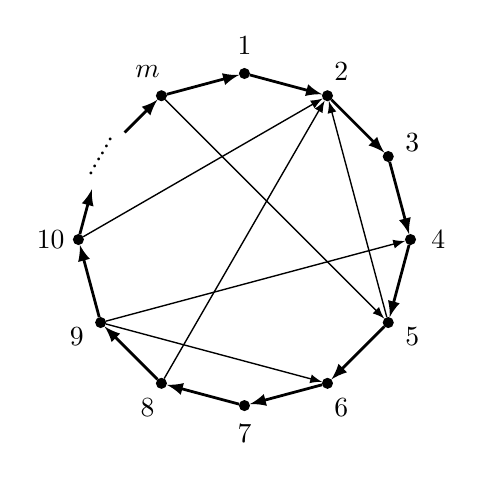
\begin{tikzpicture}
			\foreach \angle [count = \xi] in {90, 60, ..., -180}
				{
					\node[circle, fill, minimum size=.4em, inner sep=0pt, outer sep=0pt] (node\xi) at (\angle:6em) {};
					\node (nodetext\xi) at (\angle:7em) {\xi};
				}
			\node[circle, fill, minimum size=.4em, inner sep=0pt, outer sep=0pt] (node12) at (120:6em) {};
			\node (nodetext12) at (120:7em) {$m$};
			\node[rotate = 60] (node11) at (150:6em) {......};
			\draw[-latex,line width = .1em] (node12) -- (node1);
			\foreach \xi in {2, 3, ..., 12}
				{
					\pgfmathtruncatemacro\xii{\xi - 1};
					\draw[-latex,line width = .1em] (node\xii) -- (node\xi);
				}
			\foreach \x/\y in {12/5, 10/2, 8/2, 5/2, 9/4, 9/6}
				{
					\draw[-latex,line width = .05em] (node\x) -- (node\y);
				}
		\end{tikzpicture}
		 &
		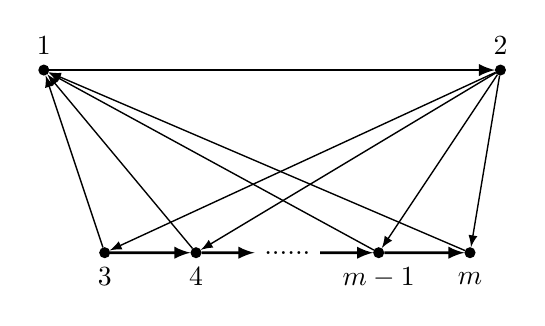
\begin{tikzpicture}[scale=1.1]
			\node[circle, fill, minimum size=.4em, inner sep=0pt, outer sep=0pt, label=above:1] (node1) {};
			\node[circle, fill, minimum size=.4em, inner sep=0pt, outer sep=0pt, label=above:2] at ([xshift = 15em]node1)(node2) {};
			\draw[-latex,line width = .1em] (node1) -- (node2);
			\node[circle, fill, minimum size=.4em, inner sep=0pt, outer sep=0pt, label=below:{3}]  at ([xshift = 2em, yshift = -6em]node1) (node31) {};
			\node[circle, fill, minimum size=.4em, inner sep=0pt, outer sep=0pt, label=below:{4}]  at ([xshift = 5em, yshift = -6em]node1) (node32) {};
			\node at ([xshift = 8em, yshift = -6em]node1) (node33) {......};
			\node[circle, fill, minimum size=.4em, inner sep=0pt, outer sep=0pt, label=below:{$m - 1$}]  at ([xshift = 11em, yshift = -6em]node1) (node34) {};
			\node[circle, fill, minimum size=.4em, inner sep=0pt, outer sep=0pt, label={[label distance = .18em]below:$m$}]  at ([xshift = 14em, yshift = -6em]node1) (node35) {};
			\foreach \i in {1, 2, 4, 5}
				{
					\draw[-latex,line width = .05em] (node2) -- (node3\i);
					\draw[-latex,line width = .05em] (node3\i) -- (node1);
				}

			\foreach \i [count = \xi] in {2, ..., 5}
				{
					\draw[-latex,line width = .1em] (node3\xi) -- (node3\i);
				}
		\end{tikzpicture}
		\\
		(a) \textsf{Aequitas}
		 &
		(b) \textsf{pompe}
		\\
	\end{tabularx}
    \addtocounter{table}{-1}
	\medskip
	
	\caption{Illustration of dependency graphs.}
	\label{fig:bad-bandwidth-illustration}
\end{figure}
